%
% API
% Abschlussarbeit (Bachelor)
%
% Thema: Erstellung einer Browser Extension zur Usability Evaluierung von beliebigen Web-Applikationen über Heatmaps.
% Betreuer 1: Prof. Dr. Targo Pavlista
% Betreuer 2: Siamak Haschemi
%
% @author Christian Bromann <contact@christian-bromann.com>
%

\newglossaryentry{URI}{name=URI, description={(Abk. für Uniform Resource Identifier) entspricht der Bedeutung der URL. Der Begriff wurde in einer späteren Spezifikation festgelegt und beschreibt die Identifikation von Ressourcen etwas allgemeinerer}}

\section{API}

Die \textbf{API} ist der Datenmotor des Frameworks. Sie ist sowohl für die Datenpersistierung als auch für dessen Auslieferung zuständig. Hinter ihr steckt eine NodeJS Applikation, die als dedizierter Service auf einem Server unter einem bestimmten Port laufen muss. Bei einem Testrun ist sie in ständiger Verbindung mit der Browser Extension, um möglichst viele Daten aufzunehmen. NodeJS eignet sich hierfür sehr gut, da es event-getrieben agiert und dabei nicht blockierend wirkt. Dies bedeutet, dass alle langandauerenden Aktivitäten, wie z.B. Dateizugriffe, Netzwerk Kommunikationen oder Datenbankzugriffe, bei Seite gepackt werden, bis sie beendet sind und das Ergebnis in einer Funktion verarbeitet werden kann \cite{nonblocking}. Dadurch werden Server-Anfragen parallel abgearbeitet und nicht, wie z.B. bei PHP, sequenziell. Dies sorgt für eine stabile Verbindung zwischen Server API und Extension. Zusätzlicher Vorteil einer NodeJS basierten API Architektur ist die Performance. NodeJS basiert auf Googles hochgeschwindigkeits V8 Engine und sorgt damit für eine deutliche höhere Reaktionszeit beim Server im Vergleich zu Apache-Servern \cite{nodevsphp}.

\subsection{Installation und Starten des Services}

Um die API auf einem Server zum Laufen zu bringen, muss NodeJS\footnote{Hinweise zur Installation von NodeJS - \url{http://nodejs.org/download/}} und Mongo\footnote{Hinweise zur Installation von MongoDB - \url{http://docs.Mongo.org/manual/installation/}} darauf installiert sein. Als Erstes erfolgt die Einrichtung der Datenbankumgebung. Mongo sollte dafür über den Befehl \textit{mongod} gestartet sein. Für die Konfiguration kann das Kommandozeileninterface des Datenbanksystems genutzt werden.

\vspace{1cm}
\begin{lstlisting}[caption=Einrichten der Mongo Datenbank,label=initMongo]
// Kommandozeileninterface starten
$ mongo

// Collection fuer thEvaluator erstellen
> db.createCollection("thEvaluator")

// zu dieser Collection wechseln
> use thEvaluator

// User anlegen
> db.addUser("username", "password")
\end{lstlisting}
\vspace{1cm}

Als nächstes sollten die Zugangsdaten für den erzeugten User in die \textit{config.json} eingetragen werden. Diese Datei enthält alle wichtigen Konfigurationsvariablen, wie z.B. der Port, auf dem die Applikation gestartet werden soll, oder Datenbankzugriffsdaten, wie Username oder Passwort. Für den Start der Applikation ist es empfehlenswert diese über das NodeJS Forever Modul zu starten. Diese kümmert sich darum, dass die App kontinuierlich im Hintergrund am Laufen gehalten wird.

\vspace{1cm}
\begin{lstlisting}[caption=Installation von Forever auf dem Server,label=forever]
$ [sudo] npm install forever -g
\end{lstlisting}
\vspace{1cm}

Nachdem dies erledigt ist und Forever erfolgreich installiert wurde, kann der nun vorhandene Kommandozeilenbefehl des Modules genutzt werden, um die NodeJS Applikation im Hintergrund starten zu lassen.

\vspace{1cm}
\begin{lstlisting}[caption=Starten des API Services über den Forever-Befehl,label=forever]
$ forever start index.js
\end{lstlisting}

\subsection{Architektur}

NodeJS bietet in seinen Core-Modulen jegliche Funktionalität, die für den Aufbau einer Anwendung notwendig ist. Zusätzlich können Packages eingebunden werden, die weitere Funktionalität für die Erstellung spezieller Anwendungen bringt. Diese sogenannten NPM\footnote{Node Packaged Modules - \url{https://npmjs.org}} Module werden von der NodeJS Community erstellt und maintained. Die API des \textit{thEvaluator} Frameworks nutzt bspw. \textit{express}\footnote{express - web application framework for node \url{http://expressjs.com/}} als Web-Applikations-Framework, um die Rest-Services zu initialisieren und die Socket Schnittstellen einzubinden. Diese werden über das \textit{Sockel.IO}\footnote{Socket.IO - v9 - \url{http://socket.io}} Modul abstrahiert. Zuletzt bietet die \textit{mongoose}\footnote{mongoose - elegant Mongo object modeling for node.js - \url{http://mongoosejs.com/}} Library eine Abstrahierung zur Mongo Datenbank. Dabei erhalten jegliche C++ - Bindings der Mongo Architektur eine entsprechende Verknüpfung mit einer JavaScript Funktion, um den Einsatz in NodeJS möglich zu machen.

\begin{center}
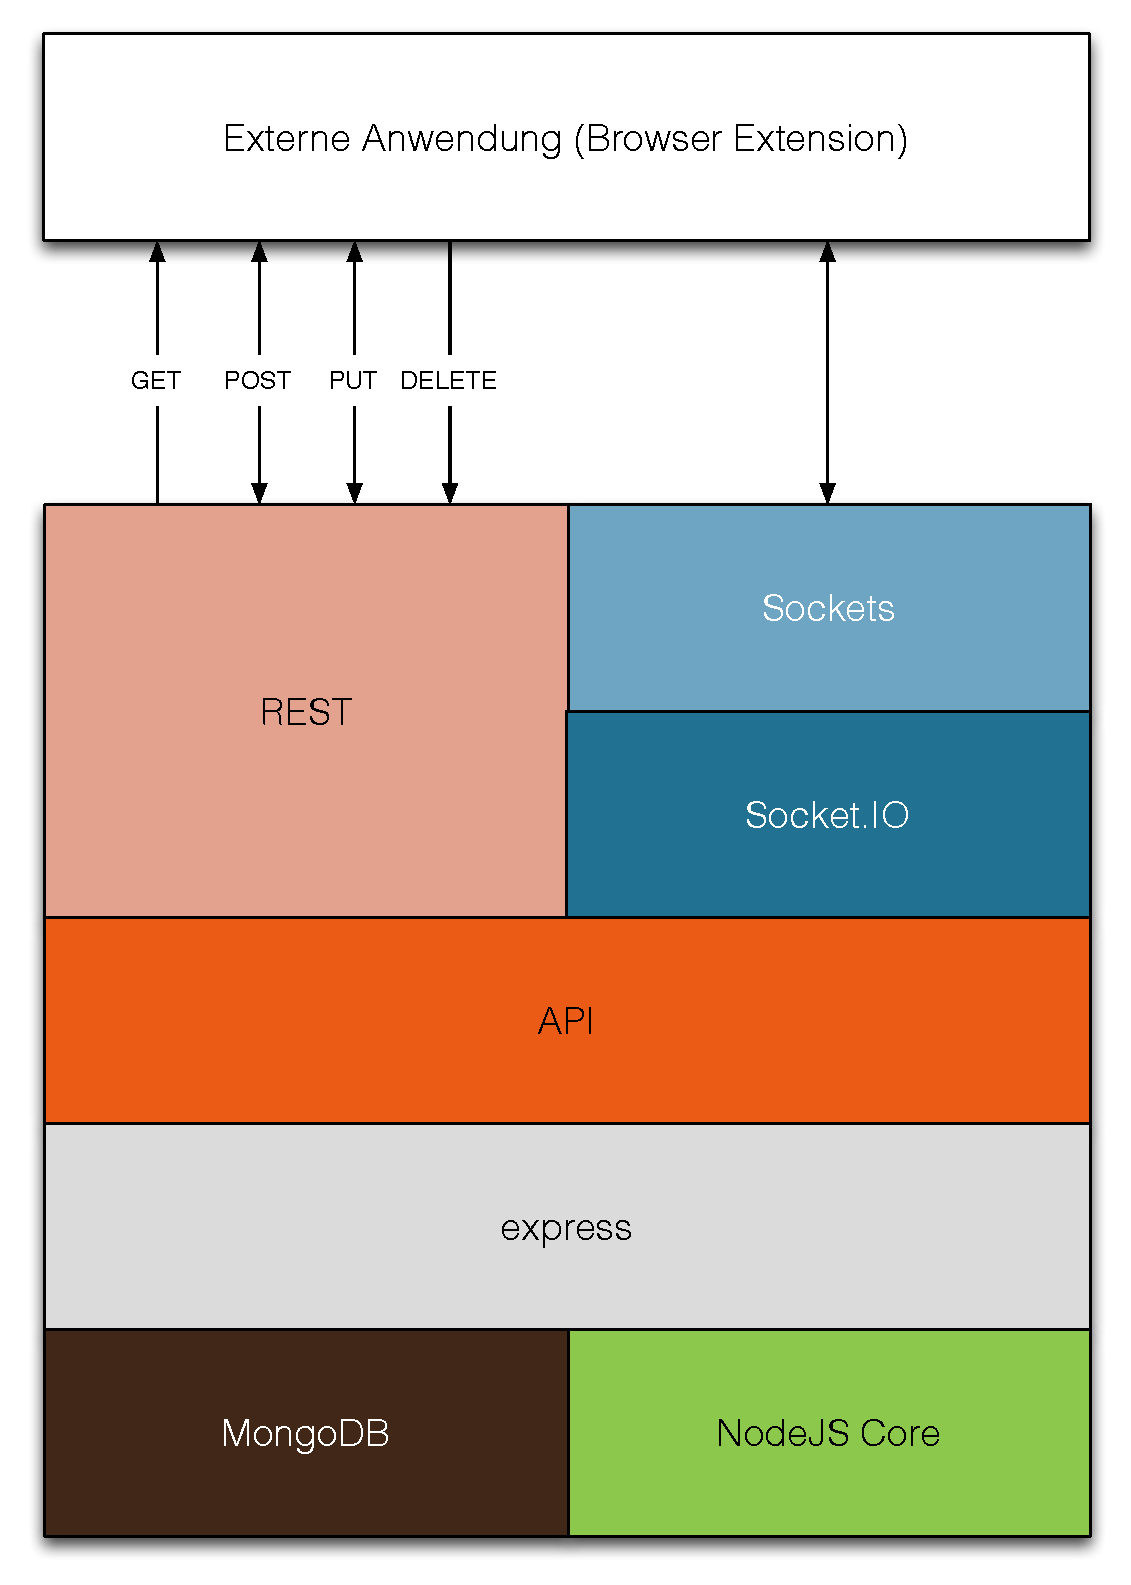
\includegraphics[scale=0.49]{./images/api-architecture}
\end{center}
\begin{figure}[htb]
   \centering
   \caption{Architektur-Schema der API}
    \label{api}
\end{figure}

Der Unterschied zwischen der Rest- und der Socket-Schnittstellen ist, dass beim Letzteren lediglich einmal eine Verbindung zwischen Client und Server hergestellt werden muss. Nach dem Handshake bleibt die TCP Verbindung bestehen und kann Daten in beide Richtungen austauschen. Der HTTP-Overhead, der teilweise mehrere 100 Byte umfassen kann, fällt dadurch weg. Da die API in der Lage sein muss viele Anfragen von der Extension aufzunehmen, spart dies enorm viel Traffic und steigert die Performance.

\subsection{Datenmodelle und Persistierung}
\label{mongo}

Wie im letzten Kapitel schon erwähnt, nutzt die API Mongo als Datenbanksystem. Mongo ist eine einfach zu skalierende, agile, dokumenten-orientierte Datenbank, geschrieben in C++. Im Bereich der NoSQL Datenbanken ist das Open Source Projekt marktführend und sehr performant. Im Gegensatz zu einer MySQL Datenbank sind die Datenstrukturen schemafrei und erforderen keine starren Tabellen mit festgelegten Spalten und Attributen. Aufgeteilt wird eine Mongo-Datenbank in verschiedene Dokumente, die unabhängig voneinander sind und getrennt auf dem Server gespeichert werden \cite{nosql}. Ein Dokument entspricht einer Tabelle einer SQL-Datenbank. Sie enthält jegliche Informationen für ein Datenobjekt. Da Mongo eine schemafreie Ansatz der Datenpersistierung verfolgt, ist die Struktur eines Dokumentes flexibel und kann immer wieder geändert werden.\\
\\
Seitdem sich NoSQL auf dem Markt etabliert hat, gibt es die Debatte darüber, welche Typ Datenbank besser ist. Viele Blog-Posts und Foren im Internet beschäftigen sich mit dem Thema und stellen letztendlich heraus, dass es keinen wirklichen Sieger in dieser Auseinandersetzung gibt. Die Wahl des Typs hängt stark von der Art der Applikation und der Vorliebe des Entwicklers ab. Für das \textit{thEvaluator} Framework fiel die Entscheidung auf MongoDB, da bereits viele positive Erfahrungen mit diesem Datenbanksystem gesammelt wurden. Sein schemaloser Charakter passt sehr gut in die dynamische Typisierung von JavaScript. Nichtsdestotrotz wäre die Persistierung der Daten in eine SQL-Datenbank ebenfalls möglich gewesen. Da die Datenobjekte ziemlich unabhängig voneinander sind, wären Argument über schlechte Performance aufgrund von vielen \textit{joins} nicht aussagekräftig gewesen.\\
\\
Obwohl MongoDB eine schemafreie Datenbank ist, erfordert es die Definition eines Schemas zur Erzeugung eines Model-Objektes. Diese Definition ist jedoch nicht verpflichtend. Die Struktur der Objekte sowie der Datentyp kann sich auch nach der initialen Erstellung ändern. Wird bspw. ein Objekt hinzugefügt, so erhalten alle schon gespeicherten Objekte den Wert \textit{null}. Dadurch erfordert es kaum Mühe und Aufwand die Datenbankstruktur zu erweitern, während die Applikation wächst.\\
\\
Die Daten des \textit{thEvaluator} Frameworks werden in vier unterschiedliche Models gespeichert. Diese beinhalten entweder eine oder mehrere Referenzen auf andere Models (in einem Array gehalten) oder speichern Daten in einer JavaScript-typisierten Form. Da MongoDB diese serialisiert in binären JSON Dateien ablegt (sog. BSON-Files), sind jegliche Typen, die JavaScript implementiert, verfügbar\footnote{der ECMAScript Standard definiert 6 verschiedene Typen: Number, String, Boolean, Null, Undefined, Object}. Datenstrukturen können somit entweder direkt als \textit{Object} im Model definiert werden oder als Referenz zu einen eigenen Modeltyp verweisen, wenn die Struktur in anderen Models ebenfalls benötigt wird.

\begin{center}
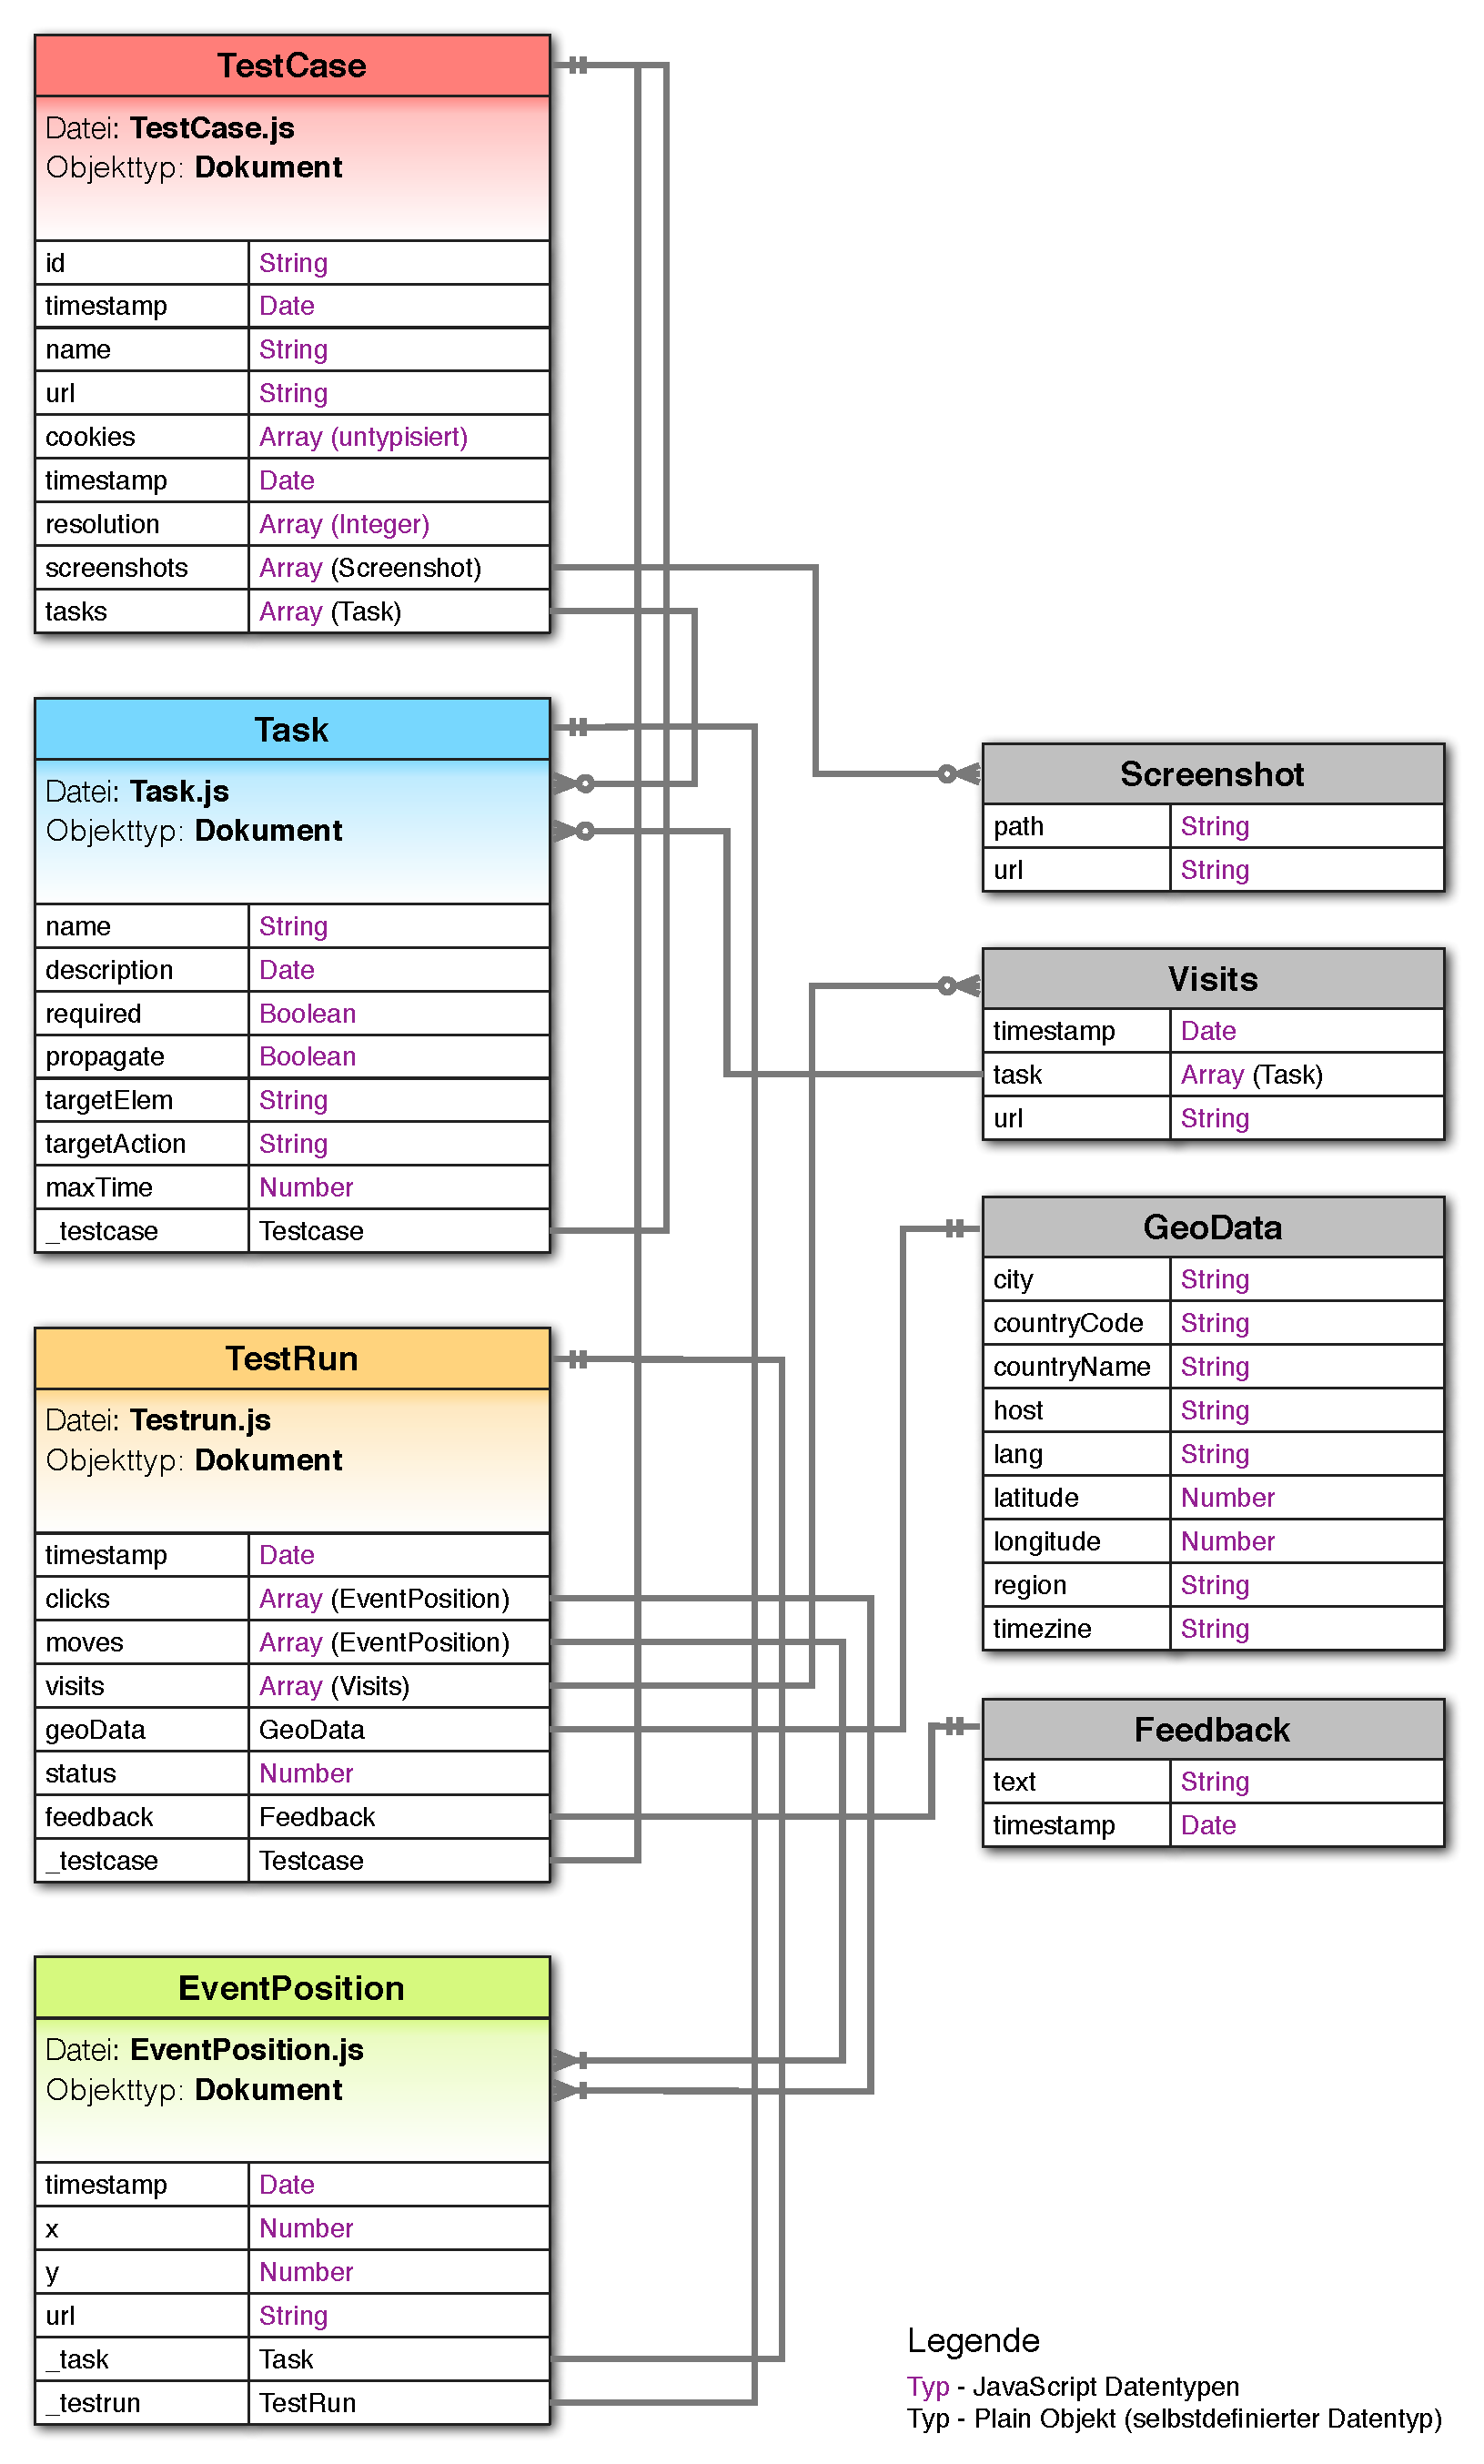
\includegraphics[scale=0.45]{./images/models}
\end{center}
\begin{figure}[htb]
   \centering
   \caption{Datenmodel der API}
    \label{models}
\end{figure}

\subsection{Asynchronität in NodeJS}

Wie zum Anfang des Kapitels beschrieben unterliegt NodeJS einer event-getriebenen und nicht blockierenden Architektur. Es wurde entwickelt von Ryan Dahl und interpretiert Java-Script in der von Google entwickelten V8 Engine. Genauso wie der Browser JavaScript lediglich in einem einzelnen Thread abarbeitet, so tut dies auch NodeJS. Es kommen keine Nebenläufigkeiten vor. Im Gegensatz zu thread-basierten Modellen, bei denen die Threads die meiste Zeit ihres Lebens im blockierten Zustand verbringen, da sie irgendwelche I/O Operationen durchführen oder eine Datenbank-Query abfragen, schiebt NodeJS seine Operationen in einen Event Loop und führt den dazugehörigen Callback erst dann aus, wenn die Operation beendet ist. Gerade bei traffic-lastigen Anwendungen, die ständig erreichbar sein müssen, sind lang blockierende Threads ein Hindernis. Während eine Operation im Event-Loop arbeitet ist NodeJS dagegen in der Lage weiterhin Anfragen anzunehmen und zu verarbeiten. Dadurch ist es perfekt geschaffen zur Erstellung von hoch skalierbaren Echtzeit-Applikationen.\\
\\
Die Methode des event-basierten Verarbeiten von Operationen, zwingt den Entwickler dabei zu einer etwas anderen Denkweise, da Operationsfolgen nicht mehr synchron sondern asynchron abgearbeitet werden müssen. Algorithmen können nicht wie gewohnt untereinander weg geschrieben werden, sondern müssen über Callbacks organisiert werden. Callbacks sind Funktionen, die aufgerufen werden, sobald eine Operation im Event Loop abgearbeitet ist. Sie enthält meist ein Error und ein Ergebnis Objekt der Operation. Listing \ref{async} zeigt ein Beispiel für asynchrone Programmierung.

\vspace{0.6cm}
\begin{lstlisting}[caption=Speichern eines Strings in eine Datei in NodeJS,label=async]
var fs = require('fs');

fs.writeFile('message.txt', 'Hello Node', function (err) {
  if (err) throw err;
  console.log('It\'s saved!');
});

console.log('saved "Hello Node" to message.txt');
\end{lstlisting}

Rein optisch betrachtet, sollte folgende Ausgabe zu erwarten sein:

\begin{verbatim}
It's saved!'
saved "Hello Node" to message.txt
\end{verbatim}

Dies ist aber nicht der Fall! Das Listing zeigt ein Script, welches das \textit{fs} Core Modul\footnote{\textit{fs} steht für File System - \url{http://nodejs.org/api/fs.html}} von NodeJS nutzt, um einen String (\glqq Hello Node\grqq{}) in die Datei \textit{message.txt} zu schreiben. Da Operationen am Dateisystem Zeit beanspruchen (wenn auch nur bruchteilhaft wenig), packt NodeJS diese in den Eventloop und hängt die als Parameter angehängte Callback Funktion an den Listener dieses Events. Dadurch wird die Funktion ausgeführt sobald die Operation beendet ist. Solange NodeJS vom Betriebssystem keine Antwort zum Bearbeitungsstand der Operation erhält, befindet diese sich in einer Art Schlafmodus. NodeJS ist daher in der Lage weiterhin Code auszuführen. Daher wird die zweite \textit{console.log} Ausgabe als erstes angezeigt und erst (bruchteilhaft) kurze Zeit später die Ausgabe aus der Callback Funktion.\\
\\
Bei komplexeren Algorithmen kann es vorkommen, dass mehrere ansynchrone Operationen hintereinander in Abhängigkeit durchgeführt werden müssen. Schnell gerät der Entwickler dabei in die missliche Lage, von zu viel ineinander geschachtelten Funktionen. Listing \ref{nested} zeigt so ein Szenario.

\vspace{0.6cm}
\begin{lstlisting}[caption=\glqq Pyramid of Doom\grqq{} - Undurchsichtiger und unsauberer Code durch zu viele verschachtelte Funktionen,label=nested]
asynchronousFunction(parameter1, function() {
  asynchronousFunction(parameter1, function() {
    asynchronousFunction(parameter1, function() {
      asynchronousFunction(parameter1, function() {
        asynchronousFunction(parameter1, function() {
          console.log('finished!');
        });
      });
    });
  });
});
\end{lstlisting}

Das Beispiel zeigt, dass der Code dadurch ziemlich schnell undurchsichtig und komplex werden kann. Führt man die ansynchronen Funktion in sequenzieller Reihenfolge aus, ist nicht einmal sicher, ob der Callback der letzten asynchronen Funktion auch wirklich als letztes ausgeführt wird.\\
\\
Um den Problemen der Asynchronität und den verschachtelten Probleme aus dem Weg zu gehen, kann man mehrere Wege gehen. Da es eine von Anfang an bestehende Thematik in NodeJS, gibt es viele Entwickler, die sich damit beschäftigt haben. Ein Lösungsansatz wäre die Nutzung von NPM Modulen, die einen Kontrollfluss abbilden, welcher die einer asynchronen nahezu gleich kommt. Einer dieser Module nennt sich \textit{Async.js}\footnote{Erläuterungen zu Async.js sind zu finden auf \url{https://github.com/caolan/async}}. Dieses hilft dem Entwickler über verschiedene Funktionen die Asynchronität zu abstrahieren und den Code mehr synchron aussehen zu lassen. Die Ausführung der Funktion geschieht zwar trotzdem noch asynchron, dennoch sieht die Struktur des Codes deutlich verständlicher aus, wie Listing \ref{asyncjs} zeigt.

\vspace{0.6cm}
\begin{lstlisting}[caption=Sequenzielle Abarbeitung von asynchronen Code durch das Async.js Module,label=asyncjs]
var async = require('async');

async.series([
    asynchronousFunction,
    asynchronousFunction,
    asynchronousFunction,
    // ...
]);
\end{lstlisting}
\vspace{0.3cm}

Das Beispiel zeigt, dass das Modul \textit{Async.js} eine Methode \textit{series} anbietet, welche eine Array mit Funktionen als Parameter aufnimmt und diese sequenziell abarbeitet. Dies ist nur eine Möglichkeit, die das Modul anbietet, um asynchrone Algorithmen so strukturieren. Es bietet für viele Varianten verschiedene Lösungen an.\\
\\
Eine weitere Möglichkeit bietet das Programmierungs-Pradigma der \glqq Promises\grqq{} in Java-Script. Als ein Promise wird ein Objekt bezeichnet, welches eine Funktion \textit{then} verlangt, die zwei Parameter entgegen nimmt \cite{promises}. Dies ist zum Einen ein \textit{success} Callback, welcher aufgerufen wird, wenn die Funktion ohne Fehler ausgeführt wurde, und zum Anderen ein \textit{failure} Callback, welcher ausgeführt wird, wenn die Funktion einen Fehler geworfen hat. Eine asynchrone Funktion liefert laut Paradigma immer ein solches Promise zurück. Die darin enthaltene \textit{then} Funktion tut dies ebenfalls wieder. Dadurch wird es möglich, beliebig viele asynchronen Funktionen miteinander zu verketten. Die Ergebnisse der jeweiligen Funktionen werden dabei immer dem Promise weitergegeben und können somit in der nächsten ansynchronen Funktion weiterverwendet werden. Listing x zeigt die Verwendung von Promises an den bisher orientierten Beispiel vom Anfang des Kapitels. 

\vspace{1.8cm}
\begin{lstlisting}[caption=Sequenzielle Abarbeitung von asynchronen Code durch das Async.js Module,label=asyncjs]
asynchronousFunction().then({
  function(data) {
    // do more asynchronous stuff
    return asynchronousFunction();
  },
  function(err) {
    throw new Error();
  }
}).then({
  function(data) {
    // do more asynchronous stuff
    return asynchronousFunction();
  }
}).then(...);
\end{lstlisting}
\vspace{0.1cm}

Durch die Bereitstellung einer \textit{then} Methode, welches die als Parameter aufgeführten Callbacks erst dann ausführt, sobald die Operation endet, ermöglichen Promises die Vereinfachungen von komplexen Asynchronen Codestrukturen. Da es noch keine offizielle Standardisierung für Promises in JavaScript gibt, wird dieses Feature in dieser Sprache noch nicht unterstützt. Mittlerweile gibt es bereits einen Vorschlag für die Spezifizierung dieses Paradigmas\footnote{CommonJS Promises/A proposal - \url{http://wiki.commonjs.org/wiki/Promises/A}}. Nach Planung von Ecma International, die EcmaScript und somit die Sprache JavaScript standardisieren, wird dieses Feature jedoch erst in EcmaScript 7 aufgenommen. Bis dahin muss sich der Entwickler auf Bibliotheken und Module verlassen, die das Paradigma versuchen abzubilden.\\
\\
Wie die Beispiele zeigen, gibt es Wege, die Asynchronität in den Griff zu bekommen. Für viele Entwickler fällt es im ersten Moment schwer, sich in die asynchrone Verarbeitung hinein zu versetzen und von den Glauben abzukommen, dass alles sequenziell abläuft. Entstehen zu viele verschachtelte Funktionen, da eine Menge asynchroner Operationen ausgeführt werden müssen, so kann es auch sein, dass NodeJS nicht das richtige Werkzeug für die Umsetzung des Vorhabens ist und sich eine thread-basierte Abarbeitung besser eignet. Diese sollte dann der Entwickler von Fall zu Fall unterscheiden.

\subsection{REST Schnittstellen}

Der als REST, oder auch \textit{\glqq REpresentational State Transfer\grqq{}}, bezeichnete Architekturstil ist ein Programmierparadigma für Webanwendungen und stellt in vielerlei Hinsicht eine retrospektive Abstraktion der Prinzipien dar, die das World Wide Web skalierbar machen \cite{rest}. Es handelt sich dabei um einen Webservice, dessen einzige Aufgabe es ist, eine bestimmte generierte Menge von Datensätzen oder Datenobjekte (representational state) für eine bestimmte \Gls{URI} bereitzustellen. Diese ist der bestimmende Faktor für den Typ und die Menge der Datensätze. Das Format der Ausgabe muss dem Client bei der Nutzung des Rest-Services bekannt sein. In den meisten Fällen handelt es sich um ein XML oder JSON Format.\\
\\
Das HTTP 1.0 Protokoll bietet vier Methoden zur Nutzung von Rest-Services an, die beschreiben, wie dieser mit den Daten umzugehen hat. Die einfachste und meist genutzte Methode ist die \textit{GET} Methode. Sie verlangt vom Server lediglich die Ausgabe der Daten. Die \textit{POST} Methode beinhaltet bei einem Request, neben der \Gls{URI}, noch Daten, die der Server aufnehmen soll. Im Erfolgsfall liefert dieser sie wieder zurück und bestätigt damit die Aufnahme der Daten in die Datenbank. Ähnlich funktioniert die \textit{PUT} Methode. Sie fügt jedoch keinen Datensatz hinzu, sondern ändert einen bestehenden. Als letztes sorgt die \textit{DELETE} Methode dafür, das ein spezieller Datensatz entfernt wird. Durch diese Methoden ist es möglich, lediglich über \Gls{URI}s, Daten in einem Rest-Service zu verwalten.\\
\\
Die API des \textit{thEvaluator} Frameworks bietet einen Rest-Service an, um die durch die Umfrage aufgenommenen Ergebnisse bereitzustellen, und die Möglichkeit zu geben, die verschiedenen Daten für Tests und Testcases zu verwalten. Genutzt wird dieser Service ausschließlich von der Webappliaktionskomponente. Für die Initialisierung der \Gls{URI}s in NodeJS ist das express Framework verantwortlich. Es bietet eine einfache Syntax für diesen Anwendungsfall an. Listing \ref{post} zeigt die Registrierung einer \Gls{URI} für die \textit{POST} Methode.

\vspace{1cm}
\begin{lstlisting}[caption=Registrierung einer URI für die \textit{POST} Methode,label=post]
var express = require('express');
var app = express();

app.post('/api/object', function(req, res){
  res.send(JSON.stringify("{...}");
});

app.listen(3000);
\end{lstlisting}
\vspace{0.6cm}

Der Callback der \textit{POST} Methode enthält zwei Parameter. Ein Request-Objekt beinhaltet zum Einen wichtige Informationen zum Request, wie z.B. Header Informationen oder mitgesendete Daten. Zum Anderen steht ein Response-Objekt bereit, das die Antwort des Servers repräsentiert. In diesem Beispiel wäre unter der URL \url{http://localhost:3000/api/object} das Objekt erreichbar, welches als Parameter in die \textit{send} Methode des Response-Objektes mitgeschickt wird. Das Listing ist lediglich eine vereinfachte Darstellung. In der Regel finden in diesen Callbacks komplexere Algorithmen und Datenbank-Abfragen statt.\\
\\
Im Folgenden gibt es eine Auflistung der angebotenen Rest-Services der API. Diese erlauben es der Webapplikation des \textit{thEvaluator} Frameworks Testcases und Tasks zu verwalten, sowie die Testergebisse einzufordern. Die Auflistung ist nach Objekttyp gruppiert.\\
\\
\\
{\footnotesize
\begin{tabular}{ p{5.5cm} p{9cm} }
  \hline
  \multicolumn{2}{c}{\textbf{Testcase}} \\
  \hline
  GET \textit{/api/testcase/:id?} & Gibt die kompletten Daten eines Testcase Objektes zurück. Ist keine ID spezifiziert, werden alle Testcases aus der Datenbank geladen\vspace{0.2cm}\\
  GET \textit{/api/testcase/:id/screenshot.jpg} & Sendet für die gegebene Testcase ID ein Screenshot im JPG Format zurück. Der Request muss dabei einen \textit{url} Parameter beinhalten mit der gewünschten URL von der Seite des Screenshots\vspace{0.2cm}\\
  POST \textit{/api/testcase} & Speicherung des Testcases, inklusive dessen Tasks, in die Datenbank\vspace{0.2cm}\\
  PUT \textit{/api/testcase/:id} & Änderung des Testcase Objektes, inklusive Inhalte und Ordnung der beinhaltenden Tasks. Eine ID des Testcases am Ende der URL wird benötigt, um einen Testcase zu spezifizieren\vspace{0.2cm}\\
  DELETE \textit{/api/testcase/:id} & Löschen eines durch die erforderliche ID spezifizierten Testcase\vspace{0.2cm}\\
  \hline
\end{tabular}
}
\\
\\
\\
{\footnotesize
\begin{tabular}{ p{5.5cm} p{9cm} }
  \hline
  \multicolumn{2}{c}{\textbf{Testrun}} \\
  \hline
  GET \textit{/api/testcase/:id?} & Gibt die kompletten Daten eines Testrun Objektes zurück. Ist keine ID spezifiziert, werden alle Testruns aus der Datenbank geladen\vspace{0.2cm}\\
  GET \textit{/api/testrun/byTestcase/:id} & Gibt die kompletten Daten eines Testrun Objektes für einen bestimmten Testcase zurück. Ist keine ID spezifiziert, werden alle Testruns des Testcases aus der Datenbank geladen\vspace{0.2cm}\\

  \hline
\end{tabular}
}
\\
\\
\\
Der Aufbau des Rest-Services ist recht simpel gehalten. Die Ausgabe der Objekte in den GET Requests erfolgt ohne Einschränkung. Das bedeutet, dass alle Attribute ausgegeben werden. Dies vereinfacht zu Beginn die Entwicklung, da sich die Webapplikation nur einmal alle Daten holen muss, um damit arbeiten zu können. Da die Applikation jedoch im Laufe der Zeit gewachsen ist und immer mehr Daten die Objekte beschreiben, werden die Ausgaben der Rest-Services immer größer. Nachdem der Beta Test von \textit{thEvaluator} gestartet war und die ersten 15 Testruns in der Produktiv-Umgebung durchgeführt wurden, stieg der Traffic zwischen Applikation und Rest-Service enorm an. Dies führte zu drastischen Performance Problemen. Der Response zur Abfrage aller Testruns eines Testcases hatte plötzlich bei einer bestimmten Testcase-ID die Größe von 8,8 MB und benötigte ca. 9 Sekunden.\\
\\
Der Rest-Service des Frameworks ist somit klar zu klein skaliert. Hier besteht eindeutig ein Verbesserungsbedarf. Objekte dürfen nicht mehr im Ganzen ausgeliefert werden, sondern sollten lediglich die Grundinformationen enthalten und Querverweise zu weiteren Daten. Diese können dann bei Bedarf über einen weiteren Request angefordert werden. Zudem sollten weitere \Gls{URI}s die Möglichkeit bieten spezielle Teile der Objekte auszulesen. Gerade bei datenlastigen Anwendungen muss es die Möglichkeit einer Art Pagination geben, da in den wenigsten Fällen wirklich alle Resultate eines Datensatzen benötigt werden.

\subsection{Socket Streams}
% Auflistung mit erforderten Werten / Rückgabewerten